\chapter{LANDASAN TEORI}

\section{Representasi Konsep dan Terminologi Klinis}

Pemetaan terminologi menyelaraskan makna istilah sumber dengan konsep dalam kosakata terkendali. Istilah merupakan bentuk bahasa, sedangkan konsep merupakan makna yang diwakili pengidentifikasi, deskripsi, dan atribut tertentu. Oleh karena itu, kesamaan kata belum menjamin kesetaraan konsep; sinonim dapat menunjuk konsep yang sama, sementara istilah serupa dapat berbeda domain atau tingkat kekhususannya \citep{cimino_desiderata_1998,schulz_stefan_interface_2017}.

\textit{Clinical data element} (CDE) dapat bersifat atomik atau komposit. CDE atomik menyatakan satu konsep utama, sedangkan CDE komposit menyertakan atribut yang memperinci makna, misalnya metode, posisi tubuh, satuan, atau kunjungan \citep{gilani_cde-mapper_2025}. Sebagai contoh, ``gula darah puasa 126 mg/dL'' memuat jenis pemeriksaan, konteks puasa, nilai, dan satuan. Nilai hasil perlu dipertahankan sebagai atribut pengamatan; pemilihan kode pemeriksaan harus mengikuti informasi yang benar-benar tersedia pada masukan.

Tiga terminologi target memiliki peran berbeda sebagaimana dirangkum pada Tabel~\ref{tab:peran-terminologi-target}. Perbedaan ini menjadi dasar pemilihan terminologi berdasarkan domain dan tujuan pemetaan, bukan kewajiban memberikan tiga kode untuk setiap entitas \citep{de_lusignan_codes_2005,schulz_stefan_interface_2017,ayuningtyas_bringing_2025}.

\begin{table}[htbp]
\centering
\small
\caption{Peran terminologi target dalam pemetaan}
\label{tab:peran-terminologi-target}
\begin{tabularx}{\textwidth}{@{}>{\raggedright\arraybackslash}p{2cm} >{\raggedright\arraybackslash}X >{\raggedright\arraybackslash}X@{}}
\toprule
\textbf{Terminologi} & \textbf{Peran} & \textbf{Implikasi pemetaan} \\
\midrule
SNOMED CT & Representasi konsep klinis dengan relasi dan atribut. & Memeriksa domain, makna, dan tingkat kekhususan konsep. \\
LOINC & Identifikasi jenis pemeriksaan atau observasi. & Mempertahankan informasi komponen, spesimen, waktu, skala, dan metode jika tersedia. \\
ICD-10 & Klasifikasi penyakit untuk agregasi dan pelaporan. & Memilih kategori sesuai diagnosis dan konteks klasifikasi. \\
\bottomrule
\end{tabularx}
\end{table}

Granularitas menyatakan tingkat kekhususan representasi. Kandidat yang lebih umum dapat kehilangan atribut, sedangkan kandidat yang lebih khusus dapat menambahkan informasi yang tidak dinyatakan sumber. Hubungan lintas terminologi juga tidak selalu berupa padanan satu-ke-satu. Karena itu, representasi konsep, status kandidat, dan atribut klinis perlu diperiksa sebelum pemetaan diterima \citep{kate_automatic_2020,huh_comparative_2025}.

\section{Normalisasi dan Ekstraksi Entitas Klinis}

Normalisasi menstandarkan bentuk teks tanpa mengubah informasi klinis yang dikandungnya. Dalam konteks Bahasa Indonesia, variasi bahasa tidak formal dan keterbatasan anotasi menjadi pertimbangan penting dalam pemrosesan teks kesehatan \citep{purwitasari_comparison_2023}. Normalisasi dalam rancangan penelitian mencakup penanganan spasi, ejaan, singkatan, dan satuan. Ekspansi singkatan memerlukan konteks; bentuk yang ambigu perlu dipertahankan atau ditandai untuk pemeriksaan. Stemming, apabila digunakan, harus dievaluasi pengaruhnya terhadap istilah klinis dan tidak diasumsikan selalu memperbaiki pemetaan.

Ekstraksi entitas mengidentifikasi bagian teks atau \textit{span} yang menyebut konsep klinis beserta tipenya. Segmentasi membagi dokumen menjadi unit pemrosesan, sedangkan ekstraksi menentukan entitas dalam unit tersebut. Pada teks panjang, pemotongan harus mempertahankan hubungan antarkalimat yang diperlukan untuk memahami entitas. Rancangan dapat menggunakan segmen bertumpang tindih, tetapi hasilnya perlu dikonsolidasikan agar entitas yang sama tidak dihitung berulang.

Representasi entitas untuk pemetaan memerlukan konteks selain nama. Integrasi NLP klinis dan pembentukan ekspresi konsep menunjukkan relevansi informasi temporal, fokus konsep, serta relasi antarkomponen \citep{hong_developing_2019,peterson_automating_2020}. Dalam penelitian ini, konteks dibedakan menjadi status pernyataan atau \textit{assertion}, waktu, dan pihak yang mengalami kondisi atau \textit{experiencer}. Sebagai contoh, ``tidak demam'', ``pernah demam'', dan ``ibu pasien demam'' memuat istilah yang sama tetapi tidak menyatakan fakta klinis yang setara tentang pasien saat ini.

Keluaran ekstraksi perlu dapat ditelusuri ke dokumen sumber melalui identitas dokumen, posisi karakter, dan bukti teks. Untuk korpus konsultasi, sumber pertanyaan pasien dan jawaban dokter dipertahankan agar diagnosis banding, rekomendasi, dan informasi umum dapat dibedakan dari fakta pasien. Rincian skema, strategi segmentasi, serta aturan validasinya merupakan bagian operasional metode pada Bab IV.

\section{LLM untuk Ekstraksi dan Dekomposisi Kueri}

Perkembangan kemampuan model bahasa pada Gambar~\ref{fig:evolusi-llm} memberikan konteks bagi penggunaan LLM untuk beberapa tugas dalam satu pipeline \citep{zhao_survey_2026}. Dalam penelitian ini, kemampuan mengikuti instruksi dan contoh dimanfaatkan untuk ekstraksi entitas, dekomposisi kueri, serta penilaian kandidat. Pemilihan model tetap didasarkan pada evaluasi tugas klinis Bahasa Indonesia, bukan pada urutan perkembangan atau ukuran model semata.

\begin{figure}[!htb]
\centering
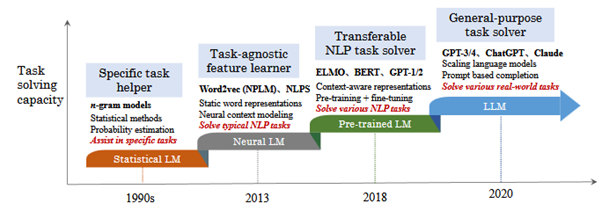
\includegraphics[width=0.85\textwidth]{media/evolusi-llm.png}
\caption[Evolusi LLM berdasarkan kemampuan penyelesaian tugas]{Evolusi LLM berdasarkan kemampuan penyelesaian tugas \citep{zhao_survey_2026}}
\label{fig:evolusi-llm}
\end{figure}

Transformer menggunakan mekanisme perhatian untuk membentuk representasi yang bergantung pada konteks \citep{vaswani_attention_2017}. Model berbasis encoder, seperti BERT, dapat digunakan untuk representasi dan klasifikasi teks; model generatif menghasilkan urutan keluaran berdasarkan masukan dan instruksi \citep{devlin_bert_2019,brown_language_2020}. Dalam pipeline penelitian ini, representasi teks diperlukan untuk pencarian semantik, sedangkan model generatif digunakan untuk ekstraksi, dekomposisi, dan penilaian kandidat. Pilihan model ditentukan oleh kebutuhan tugas dan diuji pada data pengembangan.

Gambar~\ref{fig:arsitektur-transformer} memperlihatkan arsitektur encoder--decoder Transformer, termasuk mekanisme perhatian yang menghubungkan representasi masukan dan keluaran \citep{vaswani_attention_2017}. Gambar ini menjadi landasan untuk membedakan model pembentuk representasi dan model generatif. Penggunaannya dalam penelitian tidak mensyaratkan seluruh model memiliki encoder dan decoder sekaligus; komponen yang digunakan mengikuti arsitektur model embedding atau LLM yang dipilih.

\begin{figure}[!htb]
\centering
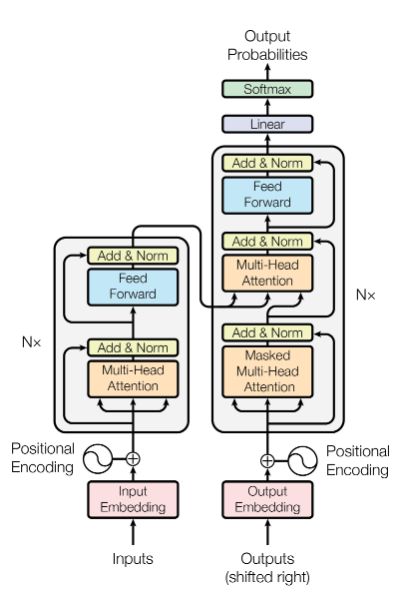
\includegraphics[width=0.75\textwidth,height=0.55\textheight,keepaspectratio]{media/arsitektur-transformer.png}
\caption[Arsitektur Transformer]{Arsitektur Transformer \citep{vaswani_attention_2017}}
\label{fig:arsitektur-transformer}
\end{figure}

\textit{In-context learning} memungkinkan model mengikuti pola tugas melalui instruksi dan contoh tanpa memperbarui parameter model. Pada \textit{few-shot prompting}, sejumlah contoh masukan--keluaran disertakan untuk memperjelas jenis entitas, atribut, serta format hasil yang diharapkan \citep{brown_language_2020}. Contoh perlu dipisahkan dari data uji. Keluaran terstruktur, seperti JSON, memudahkan pemeriksaan kelengkapan atribut dan transformasi ke tahap berikutnya, tetapi validitas format tidak membuktikan kebenaran makna.

Ekstraksi multi-entitas dan dekomposisi kueri mempunyai unit kerja berbeda. Ekstraksi mengubah satu dokumen menjadi sejumlah entitas; dekomposisi mengurai satu entitas atau CDE komposit menjadi konsep utama dan atribut pencarian. Pada CDE-Mapper, dekomposisi mencakup komponen seperti \textit{base entity}, domain, entitas terkait, kategori, satuan, dan kunjungan \citep{gilani_cde-mapper_2025}. Rancangan adaptasi menjalankan dekomposisi terhadap entitas hasil ekstraksi sambil mempertahankan identitas dan konteks sumber.

Misalnya, hasil ekstraksi ``gula darah puasa 126 mg/dL'' dapat diuraikan menjadi konsep pemeriksaan glukosa, konteks puasa, nilai 126, dan satuan mg/dL. Spesimen atau metode yang tidak disebutkan tidak boleh ditambahkan hanya untuk melengkapi struktur. Prinsip ini membatasi informasi yang boleh digunakan untuk membentuk subkueri dan menilai kandidat. Pemeriksaan bukti, validasi struktur, dan penanganan keluaran yang tidak dapat dipastikan diperlukan sebelum hasil diteruskan ke pemetaan.

\section{RAG dan Hybrid Retrieval}

\subsection{Pengambilan Pengetahuan dan Pembentukan Kandidat}

\textit{Retrieval-Augmented Generation} (RAG) menggabungkan pengambilan informasi dari sumber eksternal dengan model generatif \citep{lewis_retrieval-augmented_2021}. Pada pemetaan terminologi, sumber eksternal berupa konsep beserta deskripsi dan metadata, sedangkan keluaran yang diharapkan berupa pemilihan kandidat yang dapat ditelusuri. Secara konseptual, hubungan retriever dan generator dapat diringkas sebagai:
\begin{equation}
 p(y\mid q)=\sum_{z\in Z_k(q)}p_{\eta}(z\mid q)\,p_{\theta}(y\mid q,z),
 \label{eq:rag-probabilistic}
\end{equation}
 dengan $q$ sebagai kueri, $Z_k(q)$ sebagai konteks terambil, $p_{\eta}$ sebagai distribusi retriever, dan $p_{\theta}$ sebagai distribusi keluaran generator. Persamaan ini menjelaskan ketergantungan hasil pada konteks dan model; implementasi pemeringkatan kandidat tidak harus menghitung marginalisasi tersebut secara eksplisit.

Gambar~\ref{fig:arsitektur-rag} menunjukkan hubungan masukan, retriever, penggabungan konteks, dan generator dalam arsitektur umum RAG \citep{wu_retrieval-augmented_2025}. Dalam pemetaan terminologi, konteks eksternal berupa kandidat konsep beserta metadata, sedangkan generator digunakan untuk menilai kesesuaiannya terhadap kueri dan konteks klinis. Dengan demikian, kualitas pemetaan bergantung pada keberhasilan mengambil kandidat sekaligus kemampuan model menggunakan bukti tersebut.

\begin{figure}[!htb]
\centering
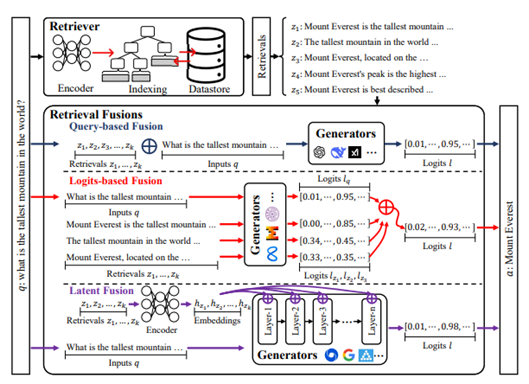
\includegraphics[width=0.9\textwidth]{media/arsitektur-rag.png}
\caption[Arsitektur umum RAG]{Arsitektur umum RAG \citep{wu_retrieval-augmented_2025}}
\label{fig:arsitektur-rag}
\end{figure}


Perbedaan Naive RAG, Advanced RAG, dan Modular RAG pada Gambar~\ref{fig:evolusi-rag} memperlihatkan perluasan alur dasar pengambilan dan pembangkitan dengan optimasi kueri, pemrosesan kandidat, serta modul yang dapat disesuaikan \citep{gao_retrieval-augmented_2024}. Bagi penelitian ini, gambaran tersebut menjelaskan penempatan normalisasi dan dekomposisi sebelum pencarian, serta filtering dan reranking setelah pencarian. Ketiga paradigma merupakan konteks konseptual; konfigurasi yang diuji tetap mengikuti rancangan eksperimen Bab IV.

\begin{figure}[!htb]
\centering
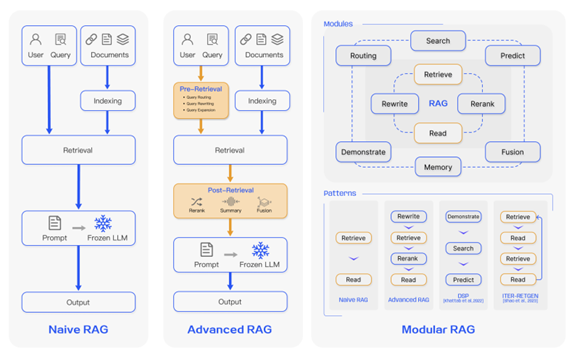
\includegraphics[width=0.9\textwidth]{media/evolusi-rag.png}
\caption[Paradigma dalam evolusi RAG]{Paradigma dalam evolusi RAG \citep{gao_retrieval-augmented_2024}}
\label{fig:evolusi-rag}
\end{figure}


CDE-Mapper mengoperasionalkan pemetaan melalui dekomposisi, retrieval, filtering, reranking, dan reservoir seperti pada Gambar~\ref{fig:framework-cde-mapper} \citep{gilani_cde-mapper_2025}. Gambar ini menunjukkan fondasi baseline; lapisan normalisasi dan ekstraksi multi-entitas Bahasa Indonesia dijelaskan dalam arsitektur adaptasi pada Bab IV.

\begin{figure}[!htb]
\centering
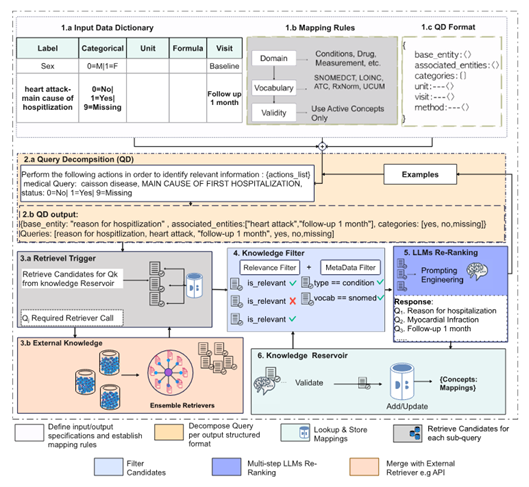
\includegraphics[width=0.9\textwidth]{media/framework-cde-mapper.png}
\caption[Framework CDE-Mapper]{Framework CDE-Mapper \citep{gilani_cde-mapper_2025}}
\label{fig:framework-cde-mapper}
\end{figure}

\subsection{Sparse, Dense, dan Penggabungan Hasil}

\textit{Dense retrieval} merepresentasikan kueri dan kandidat sebagai vektor padat. SapBERT memanfaatkan penyelarasan sinonim biomedis untuk membentuk representasi nama entitas \citep{liu_self-alignment_2021}. Kemiripan dapat dihitung dengan cosine similarity:
\begin{equation}
 s_{\mathrm{dense}}(q,c)=\frac{\mathbf{e}_{q}^{\top}\mathbf{e}_{c}}{\lVert\mathbf{e}_{q}\rVert_2\lVert\mathbf{e}_{c}\rVert_2},
 \label{eq:dense-retrieval}
\end{equation}
 dengan $\mathbf{e}_{q}$ dan $\mathbf{e}_{c}$ sebagai vektor kueri dan kandidat yang tidak bernilai nol. Kemampuan menyelaraskan sinonim biomedis tidak otomatis membuktikan kemampuan lintas bahasa untuk seluruh istilah Indonesia; kesesuaian representasinya tetap menjadi objek evaluasi.

\textit{Sparse retrieval} menggunakan representasi berbobot pada ruang kosakata $V$. SPLADE mempelajari bobot dan ekspansi leksikal dalam representasi jarang \citep{formal_splade_2021}. Skor pencocokan dinyatakan sebagai:
\begin{equation}
 s_{\mathrm{sparse}}(q,c)=\mathbf{w}_{q}^{\top}\mathbf{w}_{c}=\sum_{t\in V}w_{q,t}w_{c,t}.
 \label{eq:sparse-retrieval}
\end{equation}
 Kedua jalur menyediakan bukti yang saling melengkapi. Setelah skor disetarakan skalanya, salah satu bentuk penggabungan adalah:
\begin{equation}
 s_{\mathrm{hybrid}}(q,c)=\alpha\widetilde{s}_{\mathrm{sparse}}(q,c)+(1-\alpha)\widetilde{s}_{\mathrm{dense}}(q,c),\quad 0\leq\alpha\leq1,
 \label{eq:hybrid-retrieval}
\end{equation}
 dengan tanda tilde menyatakan skor ternormalisasi dan $\alpha$ mengatur bobot leksikal. Kandidat kemudian dipilih dari basis pengetahuan $\mathcal{K}$:
\begin{equation}
 C_k(q)=\operatorname{TopK}_{c\in\mathcal{K}}s_{\mathrm{hybrid}}(q,c).
 \label{eq:topk-candidate-set}
\end{equation}
 Penggabungan berbobot tersebut merupakan pilihan metode penelitian, bukan pernyataan tentang algoritma fusi asli CDE-Mapper. Model sparse, prosedur normalisasi skor, bobot, serta nilai $k$ harus ditetapkan dan dilaporkan dalam eksperimen.

\subsection{Routing dan Filtering}

Routing memilih ruang pencarian berdasarkan jenis entitas dan tujuan representasinya. Filtering menyaring kandidat berdasarkan metadata atau bukti kesesuaian setelah kandidat tersedia. Keduanya dapat menggunakan domain, terminologi target, status konsep, serta atribut klinis, tetapi bekerja pada titik berbeda dalam pipeline \citep{gilani_cde-mapper_2025}. Pembatasan yang terlalu ketat dapat menghilangkan kandidat benar, sedangkan pembatasan yang terlalu longgar menambah kandidat tidak relevan.

Dalam penelitian ini, diagnosis dapat memerlukan representasi klinis dan klasifikasi, sementara pemeriksaan memerlukan identifikasi observasi. Ruang pencarian karena itu dapat mencakup lebih dari satu terminologi sesuai kebutuhan. Aturan domain tidak menggantikan pemeriksaan konteks, dan skor kemiripan tidak diperlakukan sebagai probabilitas kebenaran yang telah terkalibrasi. Dampak routing dan filtering diuji melalui ablasi sebagaimana dirancang pada Bab IV.

\section{Reranking, Validasi, dan Knowledge Reservoir}

Reranking menilai ulang kandidat dengan informasi yang lebih lengkap daripada skor retrieval awal. Penilaian dapat mempertimbangkan label, sinonim, domain, atribut, serta tingkat kekhususan konsep. CDE-Mapper menggunakan penilaian relevansi dan klasifikasi hubungan kandidat, termasuk kategori exact, highly relevant, partially relevant, dan not relevant \citep{gilani_cde-mapper_2025}. Kandidat yang dekat secara semantik tetap dapat tidak tepat apabila menambahkan rincian yang tidak didukung sumber.

\textit{Self-consistency} mengagregasi beberapa keluaran untuk memperoleh keputusan yang lebih stabil \citep{wang_self-consistency_2023}. Konsistensi perlu dibedakan dari ketepatan: model dapat berulang kali menghasilkan keputusan salah. Karena itu, keputusan penerimaan dalam rancangan penelitian tetap mempertimbangkan label relevansi, konflik atribut, dan ambang penerimaan. Abstain digunakan ketika bukti belum memadai sehingga kasus memerlukan peninjauan ahli. Formula skor gabungan dan aturan penerimaan merupakan operasionalisasi model usulan pada Bab IV.

\textit{Knowledge reservoir} menyimpan pemetaan agar kasus berulang dapat menggunakan kembali hasil sebelumnya \citep{gilani_cde-mapper_2025}. Penggunaan ulang perlu memperhatikan konteks, domain, serta versi terminologi; label teks yang sama belum tentu mewakili kasus setara. Pada rancangan penelitian ini, penyimpanan pemetaan tervalidasi ahli dibedakan dari keluaran yang baru dinilai otomatis oleh LLM. Reservoir juga dibedakan dari indeks konsep untuk retrieval dan dari gold standard evaluasi.

Dengan demikian, validasi mencakup pemeriksaan format, kesesuaian terhadap bukti sumber, dan ketepatan konsep. Evaluasi reservoir memerlukan kondisi cold cache dan warm cache yang dinyatakan jelas. Data uji tidak digunakan untuk mengisi jawaban reservoir sebelum pengujian. Prinsip ini menjaga keterlacakan keputusan sekaligus memungkinkan penilaian manfaat komputasinya.

\section{Prinsip Evaluasi}

Evaluasi memisahkan ekstraksi, retrieval, dan keputusan pemetaan agar sumber kesalahan dapat diketahui. Unit evaluasi ditetapkan sebelum eksperimen: span bertipe untuk ekstraksi, pasangan entitas--terminologi untuk mapping, dan dokumen untuk evaluasi end-to-end. Gold standard, penyelesaian perbedaan anotasi, serta pembagian data dijelaskan pada Bab IV. Tabel~\ref{tab:ringkasan-metrik-evaluasi} merangkum fungsi metrik.

\begin{table}[htbp]
\centering
\small
\caption{Metrik evaluasi menurut tahap pipeline}
\label{tab:ringkasan-metrik-evaluasi}
\begin{tabularx}{\textwidth}{@{}>{\raggedright\arraybackslash}p{2.5cm} >{\raggedright\arraybackslash}X >{\raggedright\arraybackslash}X@{}}
\toprule
\textbf{Tahap} & \textbf{Metrik} & \textbf{Fokus penilaian} \\
\midrule
Ekstraksi & Precision, recall, F1; accuracy atau macro-F1 atribut. & Ketepatan span, tipe, dan konteks. \\
Retrieval & Recall@k, Top-k accuracy, MRR. & Kehadiran dan posisi kandidat benar. \\
Mapping & Accuracy@1; precision, recall, F1 end-to-end. & Ketepatan kode dan hasil pipeline. \\
Validasi & Coverage, konsistensi, agreement anotator. & Cakupan, kestabilan, dan mutu anotasi. \\
Efisiensi & Latensi, token, cache hit. & Beban komputasi dan penggunaan ulang. \\
\bottomrule
\end{tabularx}
\end{table}

\subsection{Ketepatan Ekstraksi dan Pemetaan}

Untuk $N$ kasus pemetaan yang memiliki padanan gold, akurasi kandidat utama didefinisikan sebagai:
\begin{equation}
 \mathrm{Accuracy@1}=\frac{1}{N}\sum_{i=1}^{N}\mathbf{1}(\widehat{c}_i\in G_i),
 \label{eq:accuracy}
\end{equation}
 dengan $G_i$ sebagai himpunan padanan yang diterima untuk kasus ke-$i$ dan $\widehat{c}_i$ sebagai hasil sistem. Abstain pada kasus yang memiliki padanan gold dihitung sebagai tidak benar pada ukuran ini. Akurasi bersyarat pada hasil yang diterima dilaporkan terpisah, sedangkan kasus tanpa padanan gold memerlukan evaluasi keputusan abstain tersendiri.

Pada ekstraksi, TP adalah prediksi yang cocok dengan span dan tipe gold, FP adalah prediksi yang tidak cocok, dan FN adalah entitas gold yang tidak ditemukan. Pada evaluasi end-to-end, kecocokan juga mensyaratkan kode dan terminologi target yang benar. Pencocokan dilakukan satu-ke-satu agar duplikasi prediksi tidak menambah TP.
\begin{align}
 \mathrm{Precision}&=\frac{TP}{TP+FP},\label{eq:precision}\\
 \mathrm{Recall}&=\frac{TP}{TP+FN},\label{eq:recall}\\
 F1&=\frac{2\,\mathrm{Precision}\,\mathrm{Recall}}{\mathrm{Precision}+\mathrm{Recall}}.\label{eq:f1score}
\end{align}
 Aturan kecocokan strict atau relaxed, agregasi micro atau macro, serta penanganan penyebut nol harus dinyatakan dalam protokol evaluasi. Evaluasi atribut konteks dilaporkan dengan menyebutkan apakah menggunakan entitas gold atau hanya entitas yang berhasil dicocokkan.

\subsection{Kualitas Kandidat dan Cakupan}

Jika $C_i^{(k)}$ adalah daftar Top-$k$ dan $R_i$ adalah himpunan konsep relevan, ukuran retrieval dirumuskan sebagai:
\begin{align}
 \mathrm{Top\text{-}}k\ \mathrm{Accuracy}&=\frac{1}{N}\sum_{i=1}^{N}\mathbf{1}\!\left(R_i\cap C_i^{(k)}\neq\varnothing\right),\label{eq:topk}\\
 \mathrm{Recall@}k&=\frac{1}{N}\sum_{i=1}^{N}\frac{|R_i\cap C_i^{(k)}|}{|R_i|},\label{eq:recallatk}\\
 \mathrm{MRR}&=\frac{1}{N}\sum_{i=1}^{N}\mathrm{RR}_i,\quad
 \mathrm{RR}_i=\begin{cases}1/r_i,&\text{kandidat relevan ditemukan},\\0,&\text{selainnya}.\end{cases}\label{eq:mrr}
\end{align}
 Di sini $r_i$ adalah peringkat kandidat relevan pertama. Recall@k dihitung pada kasus dengan $|R_i|>0$. Untuk satu konsep relevan per kueri, Recall@k sama dengan Top-k accuracy; untuk beberapa konsep, keduanya mengukur hal berbeda. Batas kedalaman daftar pada penghitungan MRR perlu dilaporkan.

Coverage kandidat menunjukkan proporsi masukan yang memperoleh setidaknya satu kandidat valid setelah filtering:
\begin{equation}
 \mathrm{Coverage}_{\mathrm{kandidat}}=\frac{N_{\mathrm{masukan\ dengan\ kandidat\ valid}}}{N_{\mathrm{seluruh\ masukan}}}.
 \label{eq:coverage}
\end{equation}
 Valid di sini berarti memenuhi batasan ruang pencarian, bukan telah terbukti benar menurut gold. Coverage keputusan akhir dihitung sebagai proporsi kasus yang diterima tanpa abstain dan dilaporkan terpisah. Pemisahan ini mencegah daftar kandidat yang selalu terisi dianggap sebagai keberhasilan pemetaan.

\subsection{Konsistensi, Agreement, dan Efisiensi}

Untuk $T\geq2$ pengulangan pada masukan yang sama, salah satu ukuran konsistensi adalah proporsi pasangan keputusan yang sama:
\begin{equation}
 \mathrm{Consistency}=\frac{\sum_{t<u}\mathbf{1}(L^{(t)}=L^{(u)})}{\binom{T}{2}}.
 \label{eq:consistency}
\end{equation}
 Ukuran ini dirata-ratakan pada kasus yang diuji. Ia berbeda dari proporsi suara mayoritas yang digunakan sebagai komponen skor kandidat pada Bab IV; keduanya harus dilaporkan sesuai definisinya. Konsistensi tidak menggantikan pembandingan dengan gold standard.

Kesepakatan anotator untuk keputusan kategorikal dapat dinilai dengan koefisien Kappa:
\begin{equation}
 \kappa=\frac{P_o-P_e}{1-P_e},
 \label{eq:kappa}
\end{equation}
 dengan $P_o$ sebagai kesepakatan teramati dan $P_e$ sebagai kesepakatan yang diharapkan secara kebetulan. Varian Kappa dipilih sesuai jumlah anotator dan desain penilaian. Untuk anotasi span bebas, kecocokan span dan tipe perlu diperiksa terlebih dahulu; agreement atribut dihitung pada unit yang dapat dibandingkan. Agreement anotator dan konsistensi LLM merupakan dua objek evaluasi berbeda.

Efisiensi diukur dengan waktu inferensi per unit masukan:
\begin{equation}
 \bar{t}_{\mathrm{inferensi}}=\frac{1}{N}\sum_{i=1}^{N}t_i,
 \label{eq:efficiency-time}
\end{equation}
 serta persentase pengurangan waktu terhadap baseline:
\begin{equation}
 \mathrm{Pengurangan\ waktu}(\%)=\frac{t_{\mathrm{baseline}}-t_{\mathrm{usulan}}}{t_{\mathrm{baseline}}}\times100\%.
 \label{eq:speedup}
\end{equation}

% Hindari satu baris penutup terpisah pada halaman baru.
\enlargethispage{\baselineskip}
 Nilai positif menunjukkan waktu lebih singkat; ukuran ini berbeda dari rasio speedup $t_{\mathrm{baseline}}/t_{\mathrm{usulan}}$. Perbandingan menggunakan beban kerja dan lingkungan yang sebanding, disertai jumlah panggilan LLM, penggunaan token, dan kondisi cache. Landasan evaluasi ini mendukung pengujian tiga rumusan masalah melalui pemetaan per terminologi, ekstraksi teks panjang, dan adaptasi Bahasa Indonesia pada Bab IV.


